\documentclass{../../../fal_assignment}
\graphicspath{ {../../../} }

\usepackage{amsmath}
\usepackage{enumitem}
\setlist{nosep} % Make enumerate / itemize lists more closely spaced
\usepackage[T1]{fontenc} % http://tex.stackexchange.com/a/17858
\usepackage{url}
\usepackage{todonotes}

\usepackage{listings}
\lstset{
	basicstyle=\ttfamily,
	frame=single,
	showstringspaces=false,
	breaklines=false,
	prebreak={\space\hbox{\textcolor{gray}{$\hookleftarrow$}}}
}
\lstset{
	commentstyle=\ttfamily\textit,
	keywordstyle=\ttfamily\textbf,
	stringstyle=\ttfamily,
	rulecolor=\color{black}
}
\lstset{language=C++}

\newcommand{\colvec}[2]{\begin{pmatrix}#1\\#2\end{pmatrix}}
\newcommand{\colxy}[1]{\colvec{x_{#1}}{y_{#1}}}

\title{Worksheet B}
\author{Dr Ed Powley}
\module{COMP270}
\version{1.0}

\begin{document}

\maketitle

\section*{Introduction}

In this worksheet you will use Newtonian mechanics to write an auto-aim system for a simple tank game.

Begin by \textbf{forking} the following git repository:

\begin{center}
	\url{https://github.com/Falmouth-Games-Academy/comp270-worksheet-B}
\end{center}

\textbf{Complete} the tasks described below, remembering to \textbf{commit} your work regularly.
To submit your work, open a \textbf{pull request} from your forked repository to the original repository.

\textbf{Important}: in this worksheet, you must \textbf{only} make edits to the files \texttt{controller.cpp} and \texttt{controller.h}.
Any edits to other \texttt{.cpp} or \texttt{.h} files will be \textbf{reverted} before your work is marked, regardless of whether this breaks your code!
However feel free to add as much code as necessary to \texttt{controller.cpp} and \texttt{controller.h} that makes your solutions easier to write or maintain ---
for example you are encouraged to add your own helper methods in order to enable code reuse.

\section*{Background}

\begin{figure}[ht]
	\begin{center}
		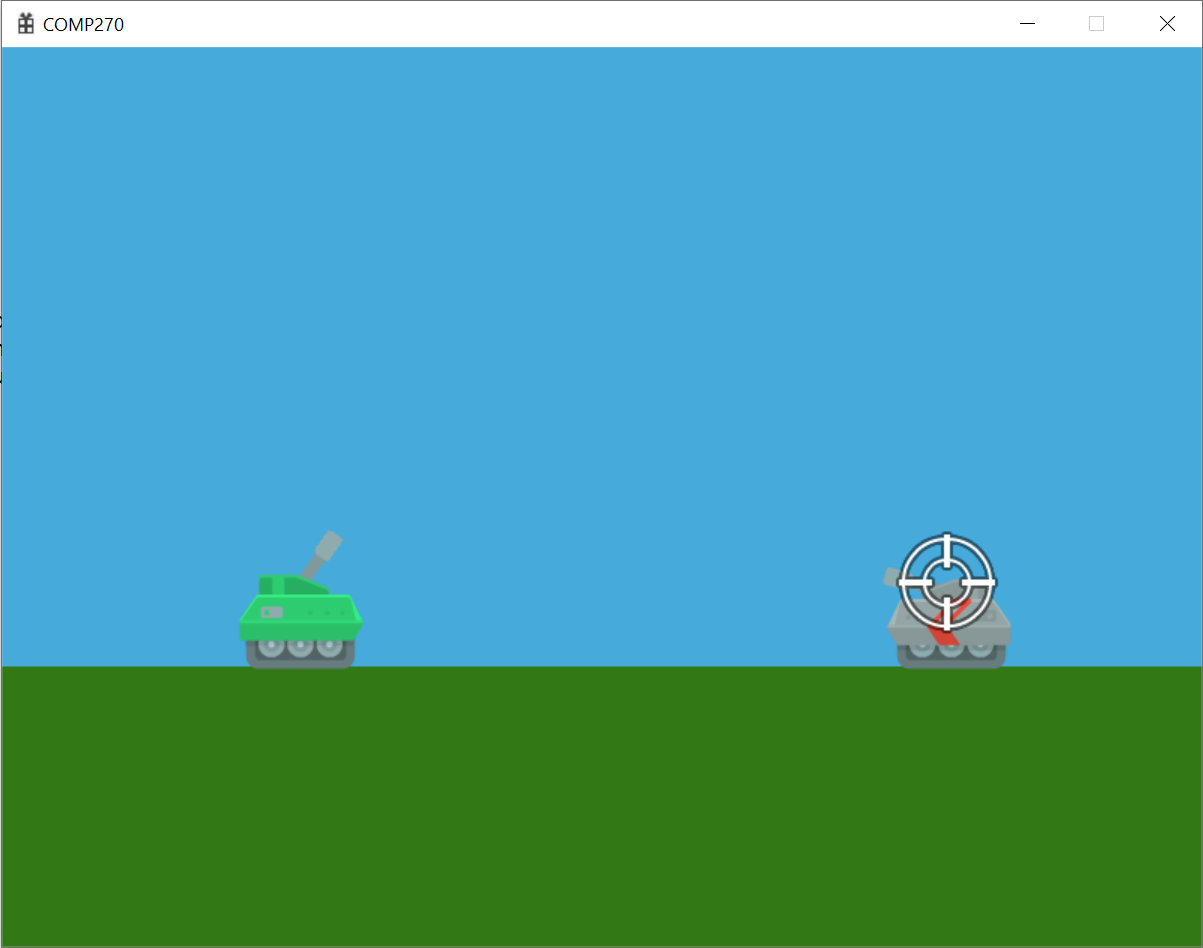
\includegraphics[width=0.7\textwidth]{game}
	\end{center}
	\caption{A screenshot of the tank game.}
	\label{fig:game}
\end{figure}

The provided skeleton project implements a simple tank combat game, as shown in Figure~\ref{fig:game}.
The player tank (green, left) and the enemy tank (grey and red, right) spawn in random positions.
On pressing the \textbf{space bar}, the player tank fires a shell with an initial speed of $u$ pixels per second, at an angle of $\theta$ radians from the horizontal (Figure~\ref{fig:shotvector}).

\begin{figure}[ht]
	\begin{center}
		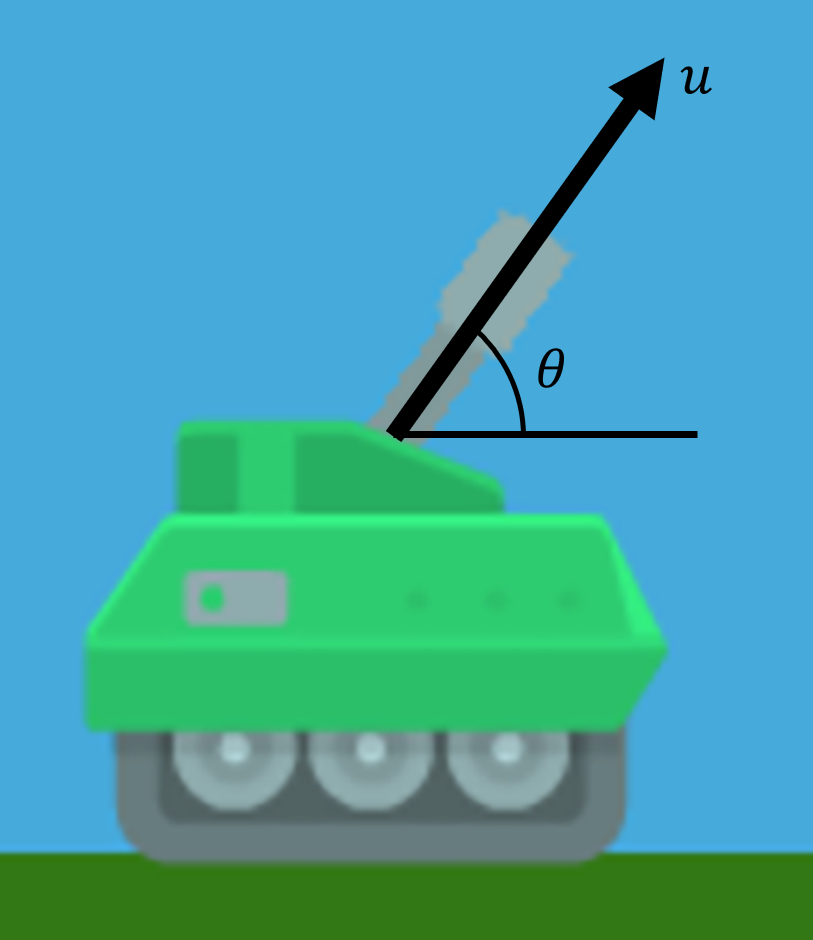
\includegraphics[width=0.5\textwidth]{shotvector}
	\end{center}
	\caption{The speed and angle of the shot.}
	\label{fig:shotvector}
\end{figure}

\section*{Task 1: calculating the shot speed}

When the shot is fired, the program calls \lstinline{Controller::calculateShotSpeed} to calculate the value of $u$.
The following information is passed in:
\begin{itemize}
	\item \lstinline{tankPos}: a vector representing the position of the tank (i.e.\ the initial position of the bullet)
	\item \lstinline{enemyPos}: the target position
	\item \lstinline{shotAngleRadians}: the angle $\theta$ in Figure~\ref{fig:shotvector}, which is fixed
	\item \lstinline{gravity}: the downward acceleration due to gravity
	\item \lstinline{wind}: for now this is always zero and can be ignored
\end{itemize}
All vectors are represented in screen space, in pixels, with the origin at the top left of the window and the positive $y$-axis pointing downwards.
Speed is represented in pixels per second, and acceleration in pixels per second per second ($\text{px} / \text{s}^2$).
The program is set up so that \lstinline{tankPos} and \lstinline{enemyPos} have the same $y$ component,
i.e.\ \lstinline{(enemyPos - tankPos).y == 0}.

\textbf{Modify} \lstinline{Controller::calculateShotSpeed} to calculate the shot speed $U$ required to hit the target.
A formula for $u$ was derived in class.

\section*{Task 2: accounting for height difference}

Edit \texttt{Controller.h} to set \lstinline{c_canHandleHeightDifference = true}.
This removes the restriction that \lstinline{tankPos} and \lstinline{enemyPos} have the same $y$ component.

\textbf{Derive} a new formula for $u$ which can handle the situation where \linebreak \lstinline{(enemyPos - tankPos).y != 0}.
\textbf{Modify} your implementation of \linebreak \lstinline{Controller::calculateShotSpeed} to use this new formula.

Note that you are \textbf{not} asked to provide your full worked derivation as part of your worksheet submission.
However make sure you include enough documentation of it in the comments for your code.

\section*{Task 3: accounting for wind}

Edit \texttt{Controller.h} to set \lstinline{c_canHandleWind = true}.
This adds a constant horizontal acceleration to the bullet, to simulate the effects of wind.
This means that the acceleration on the bullet is the vector $ \left( \begin{matrix} w \\ g \end{matrix} \right) $
where $w$ is the acceleration due to wind and $g$ is the acceleration due to gravity.
The acceleration due to wind, in $\text{px} / \text{s}^2$, is passed into \lstinline{Controller::calculateShotSpeed} as \lstinline{wind}.

\textbf{Derive} a new formula for $u$ which can handle wind.
\textbf{Modify} your implementation of \lstinline{Controller::calculateShotSpeed} to use this new formula.

\section*{Task 4: calculating the shot angle}

Edit \texttt{Controller.h} to set \lstinline{c_doCalculateAngle = true}.
Now instead of fixing the shot angle $\theta$ and calling \lstinline{Controller::calculateShotSpeed} to get the shot speed $u$,
the game fixes $u$ and calls \lstinline{Controller::calculateShotAngle} to get $\theta$.

\textbf{Derive} a formula for $\theta$ given $u$.
You may tackle the cases without height difference or wind first (by changing the relevant flags in \texttt{Controller.h} back to \lstinline{false}),
or you may tackle the general case straight away.
\textbf{Implement} your formula in \lstinline{Controller::calculateShotAngle}.

\begin{markingrubric}
	\firstcriterion{Basic competency threshold}{30\%}
		\grade\fail	A reasonable attempt at the worksheet was not submitted by the formative deadline.
	\gradespan{5}{A reasonable attempt at the worksheet was submitted by the formative deadline.
		\par		There is no evidence of academic misconduct.}
		
    \criterion{Functional coherence}{40\%}
        \grade\fail None of the tasks have been attempted.
		\grade Task 1 has been attempted and partially completed.
		\grade Task 1 has been successfully completed.
		\grade Tasks 1 and 2 have been successfully completed.
		\grade Tasks 1--3 have been successfully completed.
		\grade Tasks 1--4 have been successfully completed.

    \criterion{Maintainability}{30\%}
        \grade \fail The code is only sporadically commented, if at all, or comments are unclear.
            \par Few identifier names are clear or inappropriate.
            \par Code formatting hinders readability.
        \grade The code is well commented.
            \par Some identifier names are descriptive and appropriate.
            \par An attempt has been made to adhere to a consistent formatting style.
             \par There is little obvious duplication of code or of literal values.           
        \grade The code is reasonably well commented.
            \par Most identifier names are descriptive and appropriate.
            \par Most code adheres to a sensible formatting style.
             \par There is almost no obvious duplication of code or of literal values.   
        \grade The code is reasonably well commented, with appropriate high-level documentation.
            \par Almost all identifier names are descriptive and appropriate.
            \par Almost all code adheres to a sensible formatting style.
             \par There is no obvious duplication of code or of literal values. Some literal values can be easily ``tinkered''. 
        \grade The code is very well commented, with comprehensive appropriate high-level documentation.
            \par All identifier names are descriptive and appropriate.
            \par All code adheres to a sensible formatting style.
             \par There is no obvious duplication of code or of literal values. Most literal values are, where appropriate, easily ``tinkered''.  
        \grade The code is commented extremely well, with comprehensive appropriate high-level documentation.
            \par All identifier names are descriptive and appropriate.
            \par All code adheres to a sensible formatting style.
            \par There is no duplication of code or of literal values. Nearly all literal values are, where appropriate, easily ``tinkered''.  
\end{markingrubric}

\end{document}
